% Adapted from [MaYo26].  Regenerate: see README.md in this directory.
\documentclass[border=6pt,varwidth=16cm]{standalone}
%% Shared preamble for the figures adapted from [MaYo26]
%% (T. Makino and T. Yokoyama, RC 2026, LNCS 16626).  Copied from the
%% authors' own LaTeX source of that paper.
\usepackage[T1]{fontenc}
\usepackage{stmaryrd}
\newcommand{\sem}[1]{\llbracket #1 \rrbracket}
\usepackage{amsmath}
\usepackage{amssymb}
\usepackage{xcolor}
\pagecolor{white}
\def\pgfsysdriver{pgfsys-dvisvgm.def}
\usepackage{tikz}
\usetikzlibrary{shapes.geometric, positioning,calc}
\tikzset{
  label/.style={font=\footnotesize, font=\ttfamily},
  labelA/.style={font=\footnotesize},
  code/.style={font=\footnotesize, font=\ttfamily, text=gray},
  proc/.style={rectangle, draw, minimum size=1cm, text centered, dashed, font=\ttfamily},
  test/.style={diamond, draw, minimum size=1cm, aspect=1, text centered, font=\ttfamily},
  assert/.style={diamond, draw, minimum size=1cm, text centered, font=\ttfamily},
  asn/.style={rectangle, draw, minimum size=.5cm, text centered, font=\ttfamily},
  >=latex,
  terminal/.style={rectangle, rounded corners, draw, minimum height=6mm, text centered},
}
\renewcommand{\t}[1]{\texttt{#1}}
\newcommand{\tm}[1]{\mathtt{#1}}

\begin{document}
\[
\begin{array}{c}
(\t{E},\sigma) \to (\t{e}, (\t{E},\sigma)) \qquad \t{e}\neq\t{nil}\\
\hline
 (E_\mathrm{fss}[\raisebox{-0.7ex}{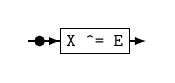
\begin{tikzpicture}[scale=.65, transform shape]
  \node[asn] (A) at (0, 0) {\texttt{X \char`^= E}}; %
  \draw[->] (A) -- ++(-1.3, 0) -- (A);
  \draw[->] (A) -- ++(1, 0);
  \fill (A.west) -- ++(-.4, 0) circle (3pt);
\end{tikzpicture}}],\sigma\uplus \{\t{X}\mapsto \t{nil}\}) \to
 (E_\mathrm{fss}[
\raisebox{-0.7ex}{\begin{tikzpicture}[scale=.65, transform shape]
  \node[asn] (A) at ($(A)+(2.5, 0)$) {\texttt{X \char`^= E}}; %
  \draw[->] (A) -- ++(-1, 0) -- (A);
  \draw[->] (A) -- ++(1.3, 0);
  \fill (A.east) -- ++(.25, 0) circle (3pt);
\end{tikzpicture}}],\sigma \uplus \{\,\t{X}\mapsto \t{e}\,\})
\end{array}~\textsc{(\textsc{AsnSet}$_\mathrm{fss}$)}
\]
\[
\begin{array}{c}
%(\t{E},\sigma,\t{d}) \to^{-1} (\t{E},\sigma')\\
(\t{E},\sigma) \to (\t{d}, (\t{E},\sigma))\\
\hline
 (E_\mathrm{fss}[\raisebox{-0.7ex}{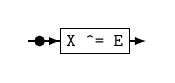
\begin{tikzpicture}[scale=.65, transform shape]
  \node[asn] (A) at (0, 0) {\texttt{X \char`^= E}}; %
  \draw[->] (A) -- ++(-1.3, 0) -- (A);
  \draw[->] (A) -- ++(1, 0);
  \fill (A.west) -- ++(-.4, 0) circle (3pt);
\end{tikzpicture}}],\sigma\uplus \{\t{X}\mapsto \t{d}\}) \to
 (E_\mathrm{fss}[
\raisebox{-0.7ex}{\begin{tikzpicture}[scale=.65, transform shape]
  \node[asn] (A) at ($(A)+(2.5, 0)$) {\texttt{X \char`^= E}}; %
  \draw[->] (A) -- ++(-1, 0) -- (A);
  \draw[->] (A) -- ++(1.3, 0);
  \fill (A.east) -- ++(.25, 0) circle (3pt);
\end{tikzpicture}}],\sigma \uplus \{\,\t{X}\mapsto \t{nil}\,\})
\end{array}~\textsc{(\textsc{AsnClear}$_\mathrm{fss}$)}
\]
\[
\begin{array}{c}
\sigma(\t{Y}) = \t{t}\\
\hline
(E_\mathrm{fss}[
\raisebox{-0.7ex}{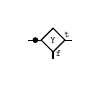
\begin{tikzpicture}[
scale=.35, transform shape,
>=,
test/.style={diamond, draw, minimum size=.3cm, aspect=1, text centered, font=\ttfamily},
]
  \node[test] (Y) {Y};

  \draw[->] (Y) -- ++(-.9, 0) -- (Y);
  \draw[->] (Y) -- ++(.7, 0);
  \node[label] at ($(Y)+(.5, .2)$) {t}; %
  \draw[->] (Y) -- ++(0, -.7);
  \node[label] at ($(Y)+(.2, -.5)$) {f}; %
  \fill (Y.west) -- ++(-.2, 0) circle (3pt);
\end{tikzpicture}}],\sigma)
\to
(E_\mathrm{fss}[
\raisebox{-0.7ex}{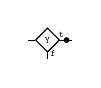
\begin{tikzpicture}[
scale=.35, transform shape,
>=,
test/.style={diamond, draw, minimum size=.3cm, aspect=1, text centered, font=\ttfamily},
]
  \node[test] (Y) {Y};

  \draw[->] (Y) -- ++(-.7, 0) -- (Y);
  \draw[->] (Y) -- ++(.9, 0);
  \node[label] at ($(Y)+(.5, .2)$) {t}; %
  \draw[->] (Y) -- ++(0, -.7);
  \node[label] at ($(Y)+(.2, -.5)$) {f}; %
  \fill (Y.east) -- ++(.25, 0) circle (3pt);
\end{tikzpicture}}],\sigma)
\end{array}
~(\textsc{TestT}_\mathrm{fss})
\quad
\begin{array}{c}
\sigma(\t{Y}) = \t{f}\\
\hline
(E_\mathrm{fss}[
\raisebox{-0.7ex}{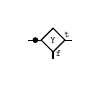
\begin{tikzpicture}[
scale=.35, transform shape,
>=,
test/.style={diamond, draw, minimum size=.3cm, aspect=1, text centered, font=\ttfamily},
]
  \node[test] (Y) {Y};

  \draw[->] (Y) -- ++(-.9, 0) -- (Y);
  \draw[->] (Y) -- ++(.7, 0);
  \node[label] at ($(Y)+(.5, .2)$) {t}; %
  \draw[->] (Y) -- ++(0, -.7);
  \node[label] at ($(Y)+(.2, -.5)$) {f}; %
  \fill (Y.west) -- ++(-.2, 0) circle (3pt);
\end{tikzpicture}}],\sigma)
\to
(E_\mathrm{fss}[
\raisebox{-0.7ex}{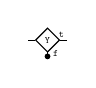
\begin{tikzpicture}[
scale=.35, transform shape,
>=,
test/.style={diamond, draw, minimum size=.3cm, aspect=1, text centered, font=\ttfamily},
]
  \node[test] (Y) {Y};

  \draw[->] (Y) -- ++(-.7, 0) -- (Y);
  \draw[->] (Y) -- ++(.7, 0);
  \node[label] at ($(Y)+(.5, .2)$) {t}; %
  \draw[->] (Y) -- ++(0, -.7);
  \node[label] at ($(Y)+(.3, -.5)$) {f}; %
  \fill (Y.south) -- ++(0,-.15) circle (3pt);
\end{tikzpicture}}],\sigma)
\end{array}
~(\textsc{TestF}_\mathrm{fss})
\]
\[
\xrightarrow{\textsc{AssertT}_\mathrm{fss}} ~~=~~ \xrightarrow{\textsc{TestT}_\mathrm{fss}}^{-1}
\qquad
\xrightarrow{\textsc{AssertF}_\mathrm{fss}} ~~=~~ \xrightarrow{\textsc{TestF}_\mathrm{fss}}^{-1}
\]
\end{document}
